\documentclass[11pt]{article}
\usepackage[a4paper,margin=1in]{geometry}
\usepackage{amsmath,amssymb}
\usepackage{graphicx}
\usepackage{booktabs}
\usepackage{siunitx}
\usepackage{subcaption}
\usepackage{hyperref}
\usepackage{float}

\title{Non-Hermitian TDVP/Arnoldi Study in \texttt{05\_arnoldi}}
\author{Project Benchmark Report}
\date{\today}

\begin{document}
\maketitle

\section{Scope and Goal}
This report documents all benchmark experiments implemented and run in \texttt{05\_arnoldi}. The central goal is to evaluate MPS-based time evolution for non-Hermitian linear ODEs,
\begin{equation}
\frac{d}{dt}\psi(t)=K\psi(t),
\end{equation}
against exact dense full-Hilbert-space references on small systems, and to compare algorithmic choices (Arnoldi vs Lanczos, TDVP vs BUG variants).

\section{Experiment Families}
\subsection{Nearest-neighbor non-Hermitian model}
Model:
\begin{equation}
K=-iJ\sum_{j=1}^{N-1} Z_jZ_{j+1} - ig\sum_{j=1}^{N}X_j - \gamma\sum_{j=1}^{N}\frac{I-Z_j}{2}.
\end{equation}
Default parameters used:
\[
N=10,\quad J=1.0,\quad g=0.7,\quad \gamma=0.2,\quad dt=0.05,\quad t_{\max}=1.0,\quad D\in\{4,8,16\}.
\]

\subsection{Long-range non-Hermitian model}
Model:
\begin{equation}
K_{\mathrm{lr}}=-i\sum_{1\le i<j\le N}J_{ij}Z_iZ_j - ig\sum_{j=1}^{N}X_j - \gamma\sum_{j=1}^{N}\frac{I-Z_j}{2},
\end{equation}
with
\begin{equation}
J_{ij}=J_0\,\lambda^{(|i-j|-1)}.
\end{equation}
Default runs used
\[
N=10,\quad J_0=1.0,\quad \lambda=0.5,\quad g=0.7,\quad \gamma=0.2,\quad dt=0.05,\quad t_{\max}=1.0,\quad D\in\{4,8,16,32\}.
\]
Additional sweeps included \(\lambda\in\{0.25,0.5,0.75\}\) for BUG-vs-TDVP comparisons.

\subsection{Exact reference}
For all benchmarks, the reference is dense full-space evolution:
\[
U=\exp(dt\,K),\qquad \psi_{n+1}=U\psi_n.
\]
No tensor-train compression is used in the reference.

\section{Implementation Notes}
\subsection{TDVP entry point and Krylov switch}
The repository's existing routines were used:
\begin{itemize}
  \item \texttt{Yaqs.Algorithms.two\_site\_tdvp!}
  \item \texttt{Yaqs.Algorithms.set\_krylov\_ishermitian\_mode!}
\end{itemize}

Because TDVP internally applies local propagators of the form \(\exp(-i\,dt\,A)\), the experiment passes
\[
A=iK
\]
to realize target dynamics \(\exp(dt\,K)\).

\subsection{Krylov mode behavior check}
Direct test results:
\begin{itemize}
  \item Forced \texttt{:lanczos} does \emph{not} auto-switch and stays in Lanczos mode.
  \item \texttt{:auto} on the non-Hermitian problem switches to Arnoldi.
\end{itemize}
Therefore, using \texttt{--krylov lanczos} explicitly forces a method that is not appropriate for this non-Hermitian case.

\section{Key Results}
\subsection{Nearest-neighbor, Arnoldi TDVP}
From \texttt{results/summary.txt}:
\begin{center}
\begin{tabular}{@{}lcc@{}}
\toprule
Bond dim \(D\) & Final state error \(\|\psi_{\mathrm{tdvp}}-\psi_{\mathrm{ref}}\|_2\) & Final max local error \(\max_j|\Delta\langle Z_j\rangle|\) \\
\midrule
4  & \(4.68\times 10^{-4}\) & \(5.79\times 10^{-6}\) \\
8  & \(4.59\times 10^{-6}\) & \(2.69\times 10^{-7}\) \\
16 & \(4.59\times 10^{-6}\) & \(2.69\times 10^{-7}\) \\
\bottomrule
\end{tabular}
\end{center}
Accuracy saturates already around \(D=8\) for this setup.

\subsection{Long-range, Arnoldi TDVP (\(\lambda=0.5\))}
From \texttt{results\_longrange/summary.txt}:
\begin{center}
\begin{tabular}{@{}lcc@{}}
\toprule
Bond dim \(D\) & Final state error & Final max local error \\
\midrule
4  & \(4.86\times 10^{-2}\) & \(3.94\times 10^{-4}\) \\
8  & \(3.31\times 10^{-3}\) & \(2.50\times 10^{-5}\) \\
16 & \(5.67\times 10^{-4}\) & \(3.24\times 10^{-5}\) \\
32 & \(5.66\times 10^{-4}\) & \(3.24\times 10^{-5}\) \\
\bottomrule
\end{tabular}
\end{center}
Long-range dynamics are harder, but Arnoldi TDVP remains accurate and converges with \(D\).

\subsection{Arnoldi vs Lanczos for non-Hermitian evolution}
Observed behavior:
\begin{itemize}
  \item Arnoldi: stable and accurate.
  \item Lanczos (forced): large persistent errors (\(\sim 10^{-1}\) to \(10^{0}\) scale), many non-Hermitian warnings.
\end{itemize}
Conclusion: for this non-Hermitian class, Arnoldi is clearly the correct Krylov choice.

\subsection{TDVP vs BUG (second-order variants)}
Comparison runs in \texttt{results\_bug2\_compare/summary.txt} show:
\begin{itemize}
  \item TDVP (Arnoldi) improves strongly with \(D\) across nearest-neighbor and long-range cases.
  \item BUG-based trajectories (both original and non-Hermitian-adapted variant tested) stayed at much larger errors and did not improve meaningfully with \(D\) in this benchmark suite.
\end{itemize}

\section{Selected Plots}
\begin{figure}[H]
    \centering
    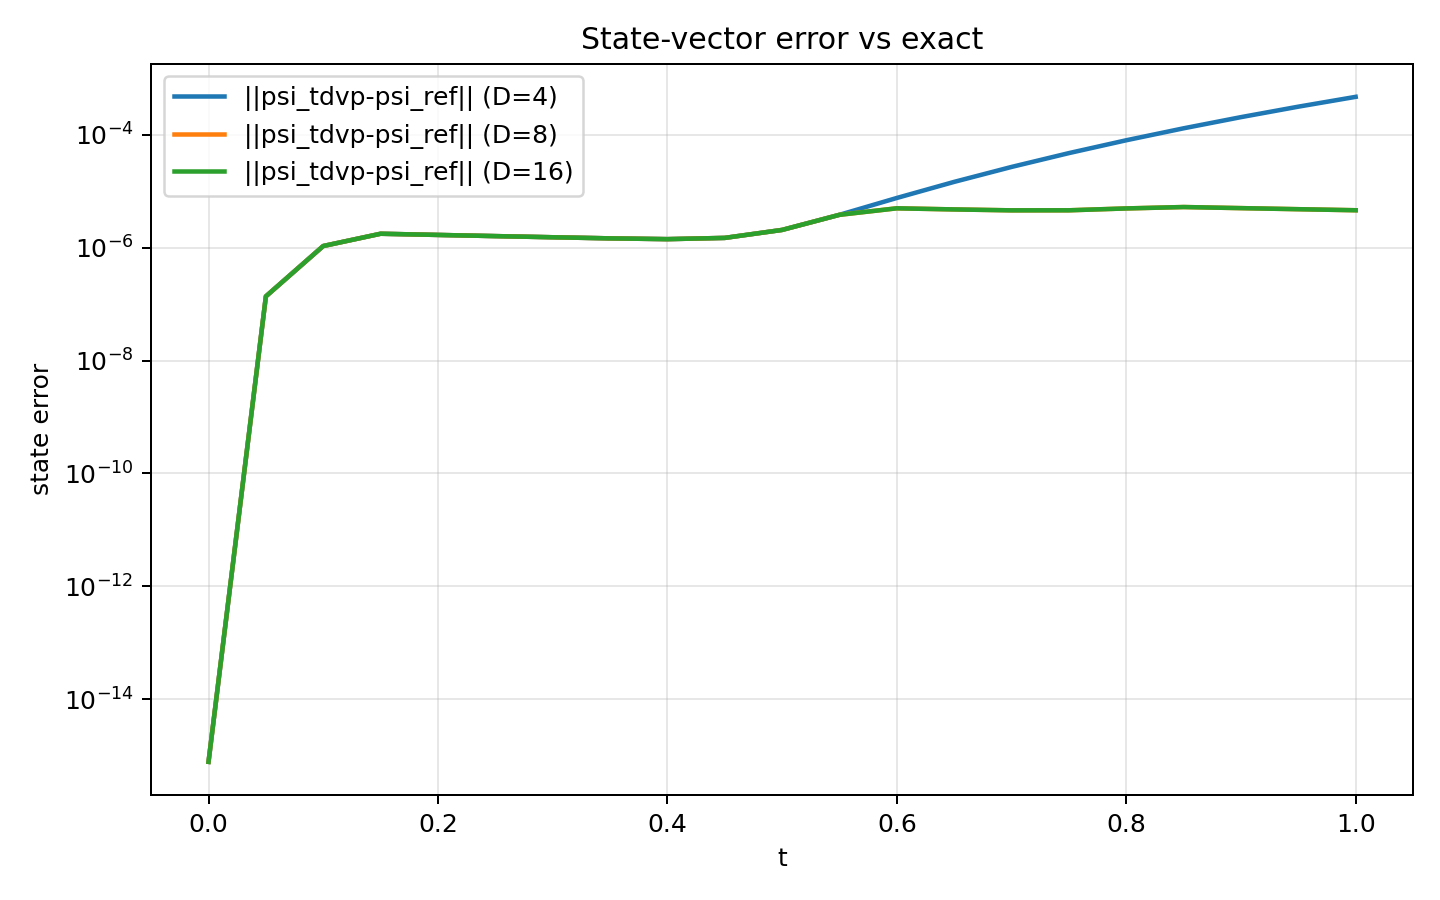
\includegraphics[width=0.75\textwidth]{results/comparison_state_error.png}
    \caption{Nearest-neighbor benchmark: TDVP state error vs exact reference.}
\end{figure}

\begin{figure}[H]
    \centering
    
\includegraphics[width=0.75\textwidth]{{results_longrange/comparison_state_error_lambda0.5}.png}
    \caption{Long-range benchmark (\(\lambda=0.5\)): TDVP state error vs exact reference.}
\end{figure}

\begin{figure}[H]
    \centering
    \begin{subfigure}{0.49\textwidth}
        \centering
        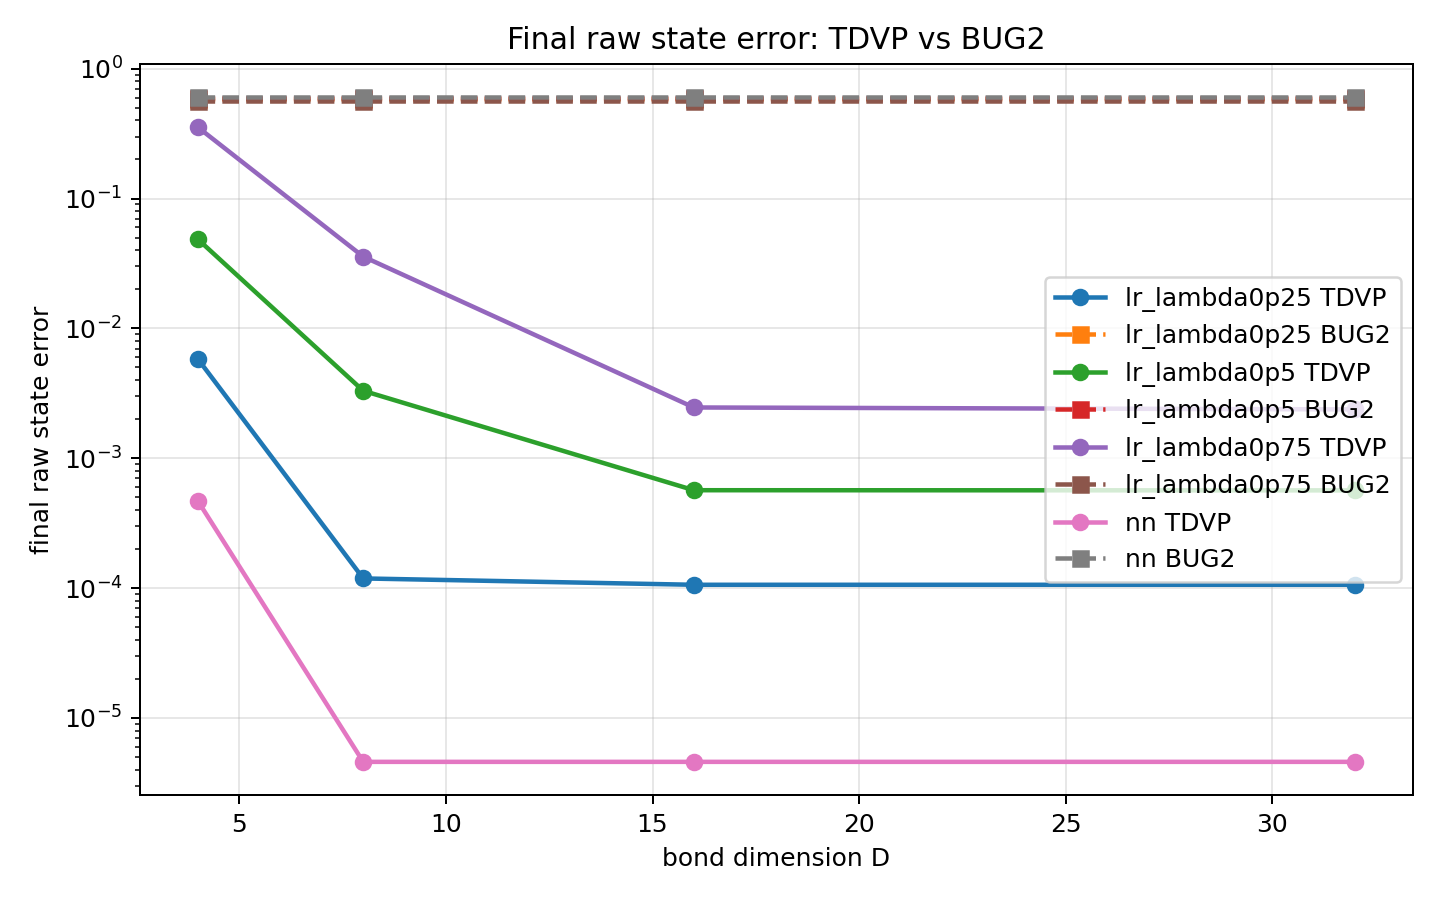
\includegraphics[width=\textwidth]{results_bug2_compare/bug2_vs_tdvp_final_error_raw.png}
        \caption{Raw final state error}
    \end{subfigure}
    \hfill
    \begin{subfigure}{0.49\textwidth}
        \centering
        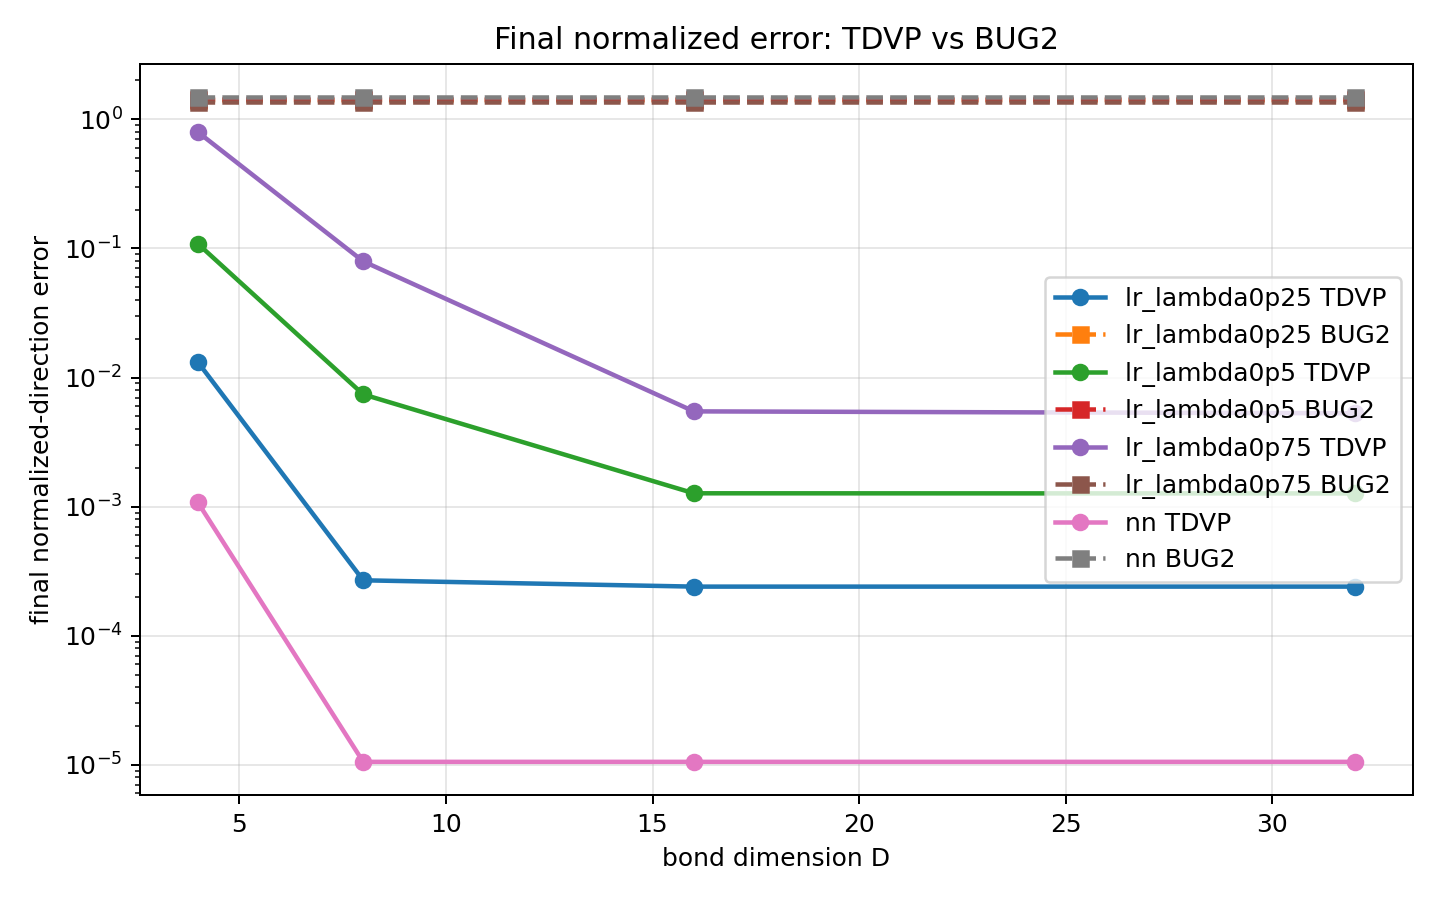
\includegraphics[width=\textwidth]{results_bug2_compare/bug2_vs_tdvp_final_error_normed.png}
        \caption{Normalized-direction final error}
    \end{subfigure}
    \caption{TDVP vs BUG comparisons across models and bond dimensions.}
\end{figure}

\begin{figure}[H]
    \centering
    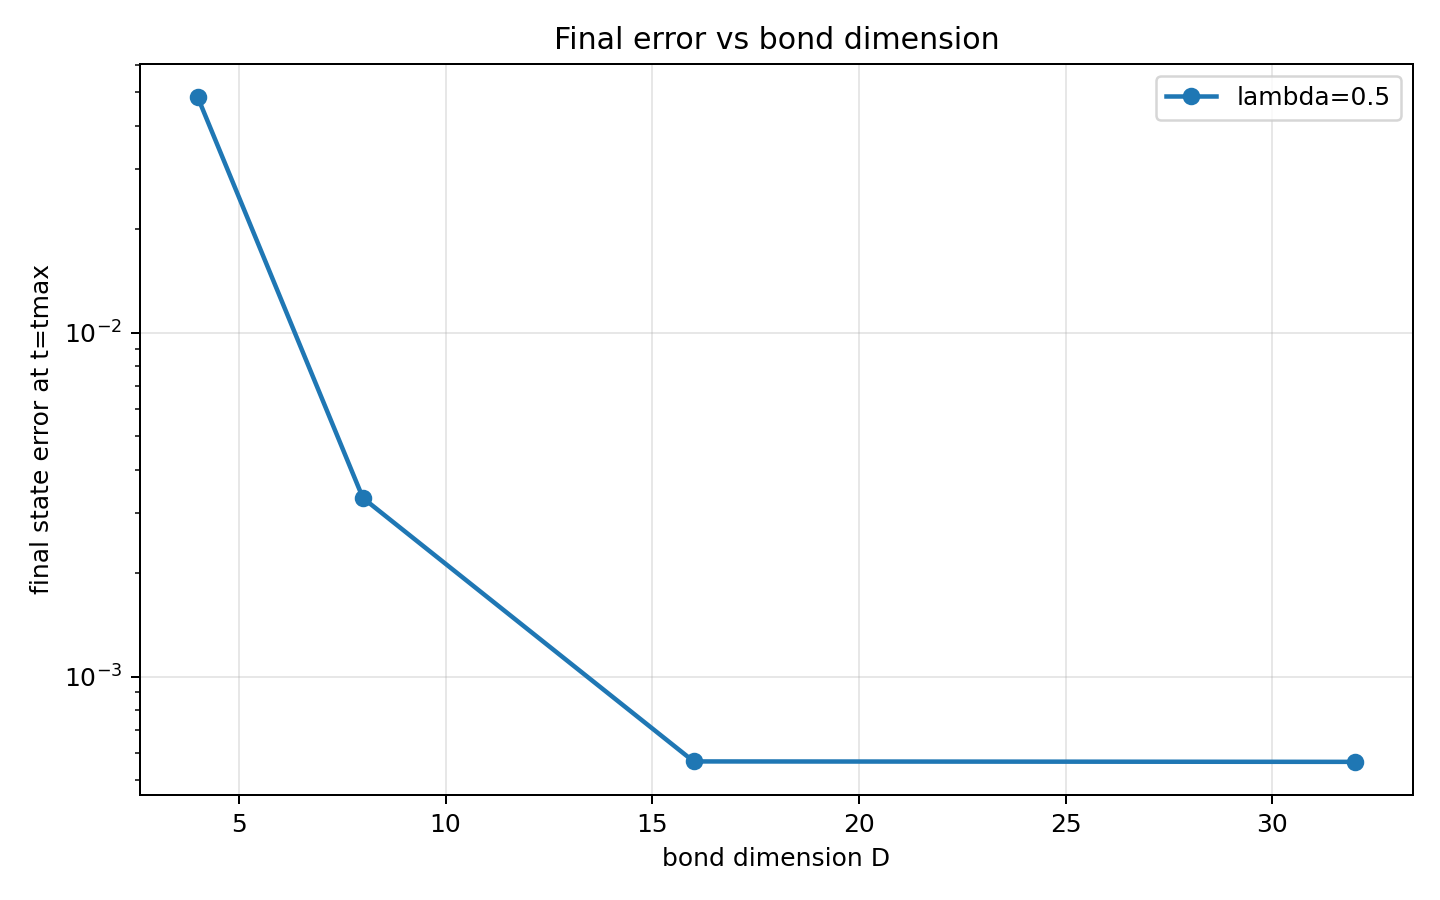
\includegraphics[width=0.75\textwidth]{results_longrange/final_error_vs_D.png}
    \caption{Long-range TDVP: final error vs bond dimension \(D\).}
\end{figure}

\section{Conclusions}
\begin{itemize}
  \item The benchmark infrastructure in \texttt{05\_arnoldi} successfully validates non-Hermitian TDVP against exact dense references.
  \item Arnoldi is the preferred Krylov mode for these non-Hermitian operators.
  \item Forced Lanczos is not suitable in this setting and should not be used for production non-Hermitian runs.
  \item In this benchmark suite, BUG variants were consistently inferior to Arnoldi-TDVP.
\end{itemize}

\section{Outlook / Next Steps}
Potential follow-up directions:
\begin{enumerate}
  \item \textbf{Higher-system-size scaling:} increase \(N\) while replacing dense exact reference by controlled high-\(D\) reference windows to extend the regime.
  \item \textbf{Adaptive tolerances:} tune Krylov tolerance and truncation thresholds jointly, report accuracy/runtime Pareto fronts.
  \item \textbf{Observable-focused validation:} add nonlocal observables (two-point correlators, structure factors) in addition to local \(\langle Z_j\rangle\).
  \item \textbf{Non-Hermitian stress tests:} sweep \(\gamma\), \(\lambda\), and stronger long-range couplings; map where a given \(D\) ceases to be reliable.
  \item \textbf{Method development branch:} if BUG remains of interest, prototype a truly non-Hermitian-targeted BUG variant (without implicit normalization effects) in an isolated branch and benchmark again against the same suite.
\end{enumerate}

\end{document}
